% Regenerate from this directory (LaTeX and dvisvgm):
% latex -interaction=nonstopmode -halt-on-error hld-2.tex
% dvisvgm --no-fonts --exact --bbox=papersize hld-2.dvi -o hld-2.svg
\documentclass[tikz,border=6pt]{standalone}
\usepackage{tikz}
\usepackage{amsmath}
\usetikzlibrary{decorations.pathreplacing,calc}
\definecolor{chaincolor}{HTML}{E62C30}
\definecolor{distancecolor}{HTML}{16A34A}
\definecolor{subtreecolor}{HTML}{ECAA00}
\definecolor{bracecolor}{HTML}{527FD0}
\begin{document}
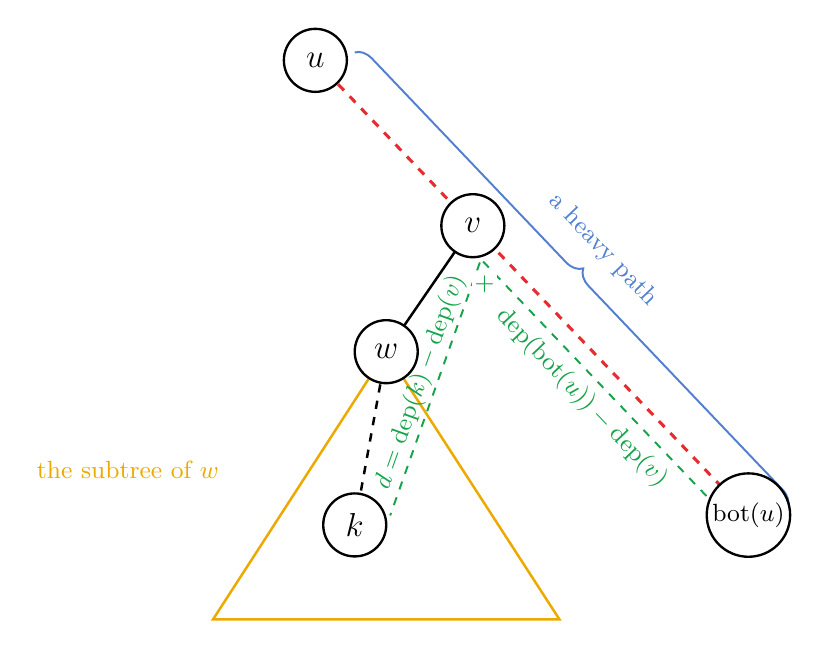
\begin{tikzpicture}[
  vertex/.style={circle,draw=black,line width=.85pt,fill=white,
    minimum size=8mm,inner sep=1pt,font=\large},
  querydistance/.style={distancecolor,dashed,line width=.7pt},
]
  \coordinate (u) at (0,0);
  \coordinate (v) at (2,-2.1);
  \coordinate (w) at (.9,-3.7);
  \coordinate (k) at (.5,-5.9);
  \coordinate (bottom) at (5.5,-5.775);
  % The queried vertex k lies in the subtree of w, a light child of v.
  \draw[subtreecolor,line width=.9pt] (w)--(-1.3,-7.1)--(3.1,-7.1)--cycle;
  \node[text=subtreecolor,anchor=east,font=\small] at (-1.1,-5.2)
    {the subtree of $w$};
  \draw[black,line width=.9pt] (v)--(w);
  \draw[black,dashed,line width=.9pt] (w)--(k);
  % u, v, and bot(u) are on one heavy chain. The two green distances
  % sum to the result of querying dis(k, bot(u)).
  \draw[chaincolor,dashed,line width=1.1pt] (u)--(v)--(bottom);
  \draw[querydistance] ($(v)+(-.16,-.15)$)--($(bottom)+(-.16,-.15)$)
    node[midway,sloped,below,font=\small]
    {$\operatorname{dep}(\operatorname{bot}(u))-\operatorname{dep}(v)$};
  \draw[querydistance] ($(v)+(.23,-.07)$)--($(k)+(.45,.12)$)
    node[pos=.55,sloped,above,inner sep=1pt,font=\small]
    {$d=\operatorname{dep}(k)-\operatorname{dep}(v)$};
  \node[text=distancecolor,fill=white,inner sep=1pt,font=\small]
    at ($(v)+(.15,-.75)$) {$+$};
  \draw[bracecolor,line width=.7pt,decorate,decoration={brace,amplitude=6pt}]
    ($(u)+(.5,.1)$)--($(bottom)+(.5,.1)$)
    node[midway,sloped,above=8pt,font=\small] {a heavy path};
  \node[vertex] at (u) {$u$};
  \node[vertex] at (v) {$v$};
  \node[vertex] at (w) {$w$};
  \node[vertex] at (k) {$k$};
  \node[vertex,font=\small] at (bottom) {$\operatorname{bot}(u)$};
\end{tikzpicture}
\end{document}
